In the current 4G and 5G communication system, the spectrum band utilized is 
competing with that of the radar system below 10 GHz, leading to severe 
spectrum congestion and hinder the performance of both future communication 
and radar system \cite{liu2020road}. Communications and Radar Spectrum Sharing (CRSS) was proposed to enable 
the two systems to perform in the same frequency band with tiny performance loss, 
which is regarded as the long-term solution for the spectrum management of 
communications and radar \cite{liu2020tutorial,feng2020survey}. Designing a dual-functional 
radar and communication (DFRC) system is one of the most popular aspects of the literature.

\begin{figure}[htbp]
    \centering
    \subfigure[Separated Deployment]{
        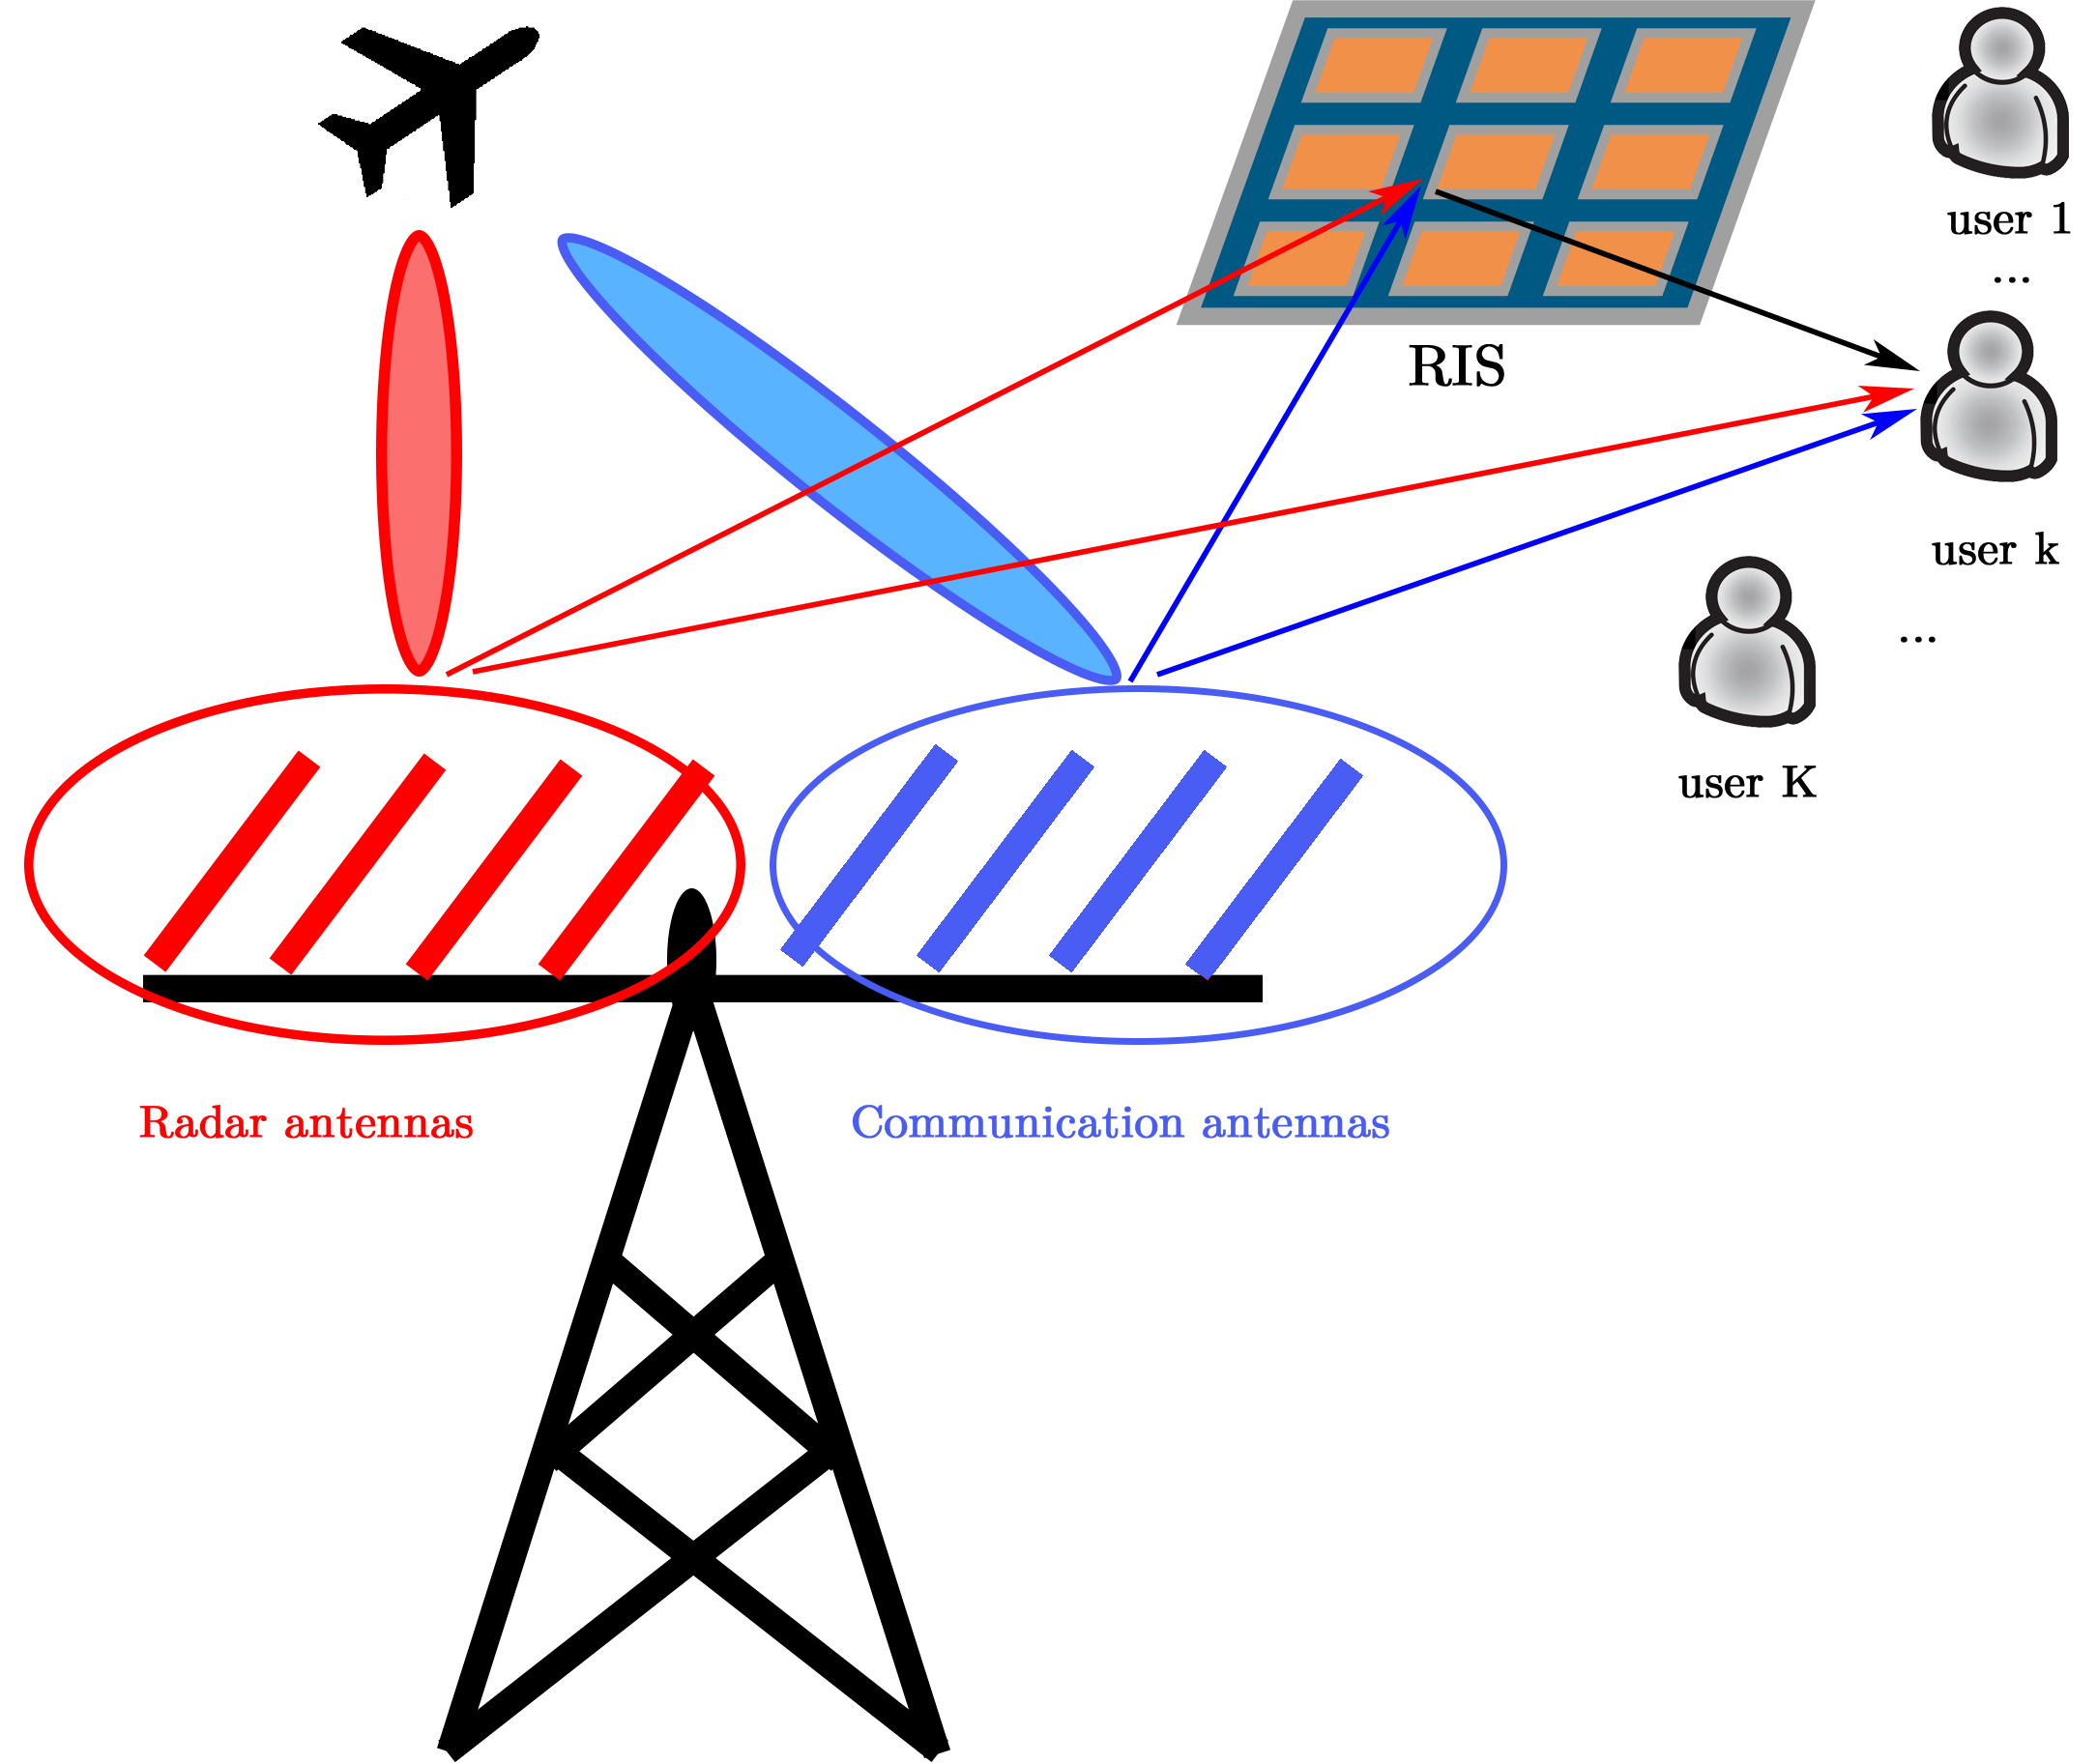
\includegraphics[width=0.42\textwidth]{./separated_setup.png}
        \label{fig:setup_separated}
    }
    \subfigure[Shared Deployment]{
	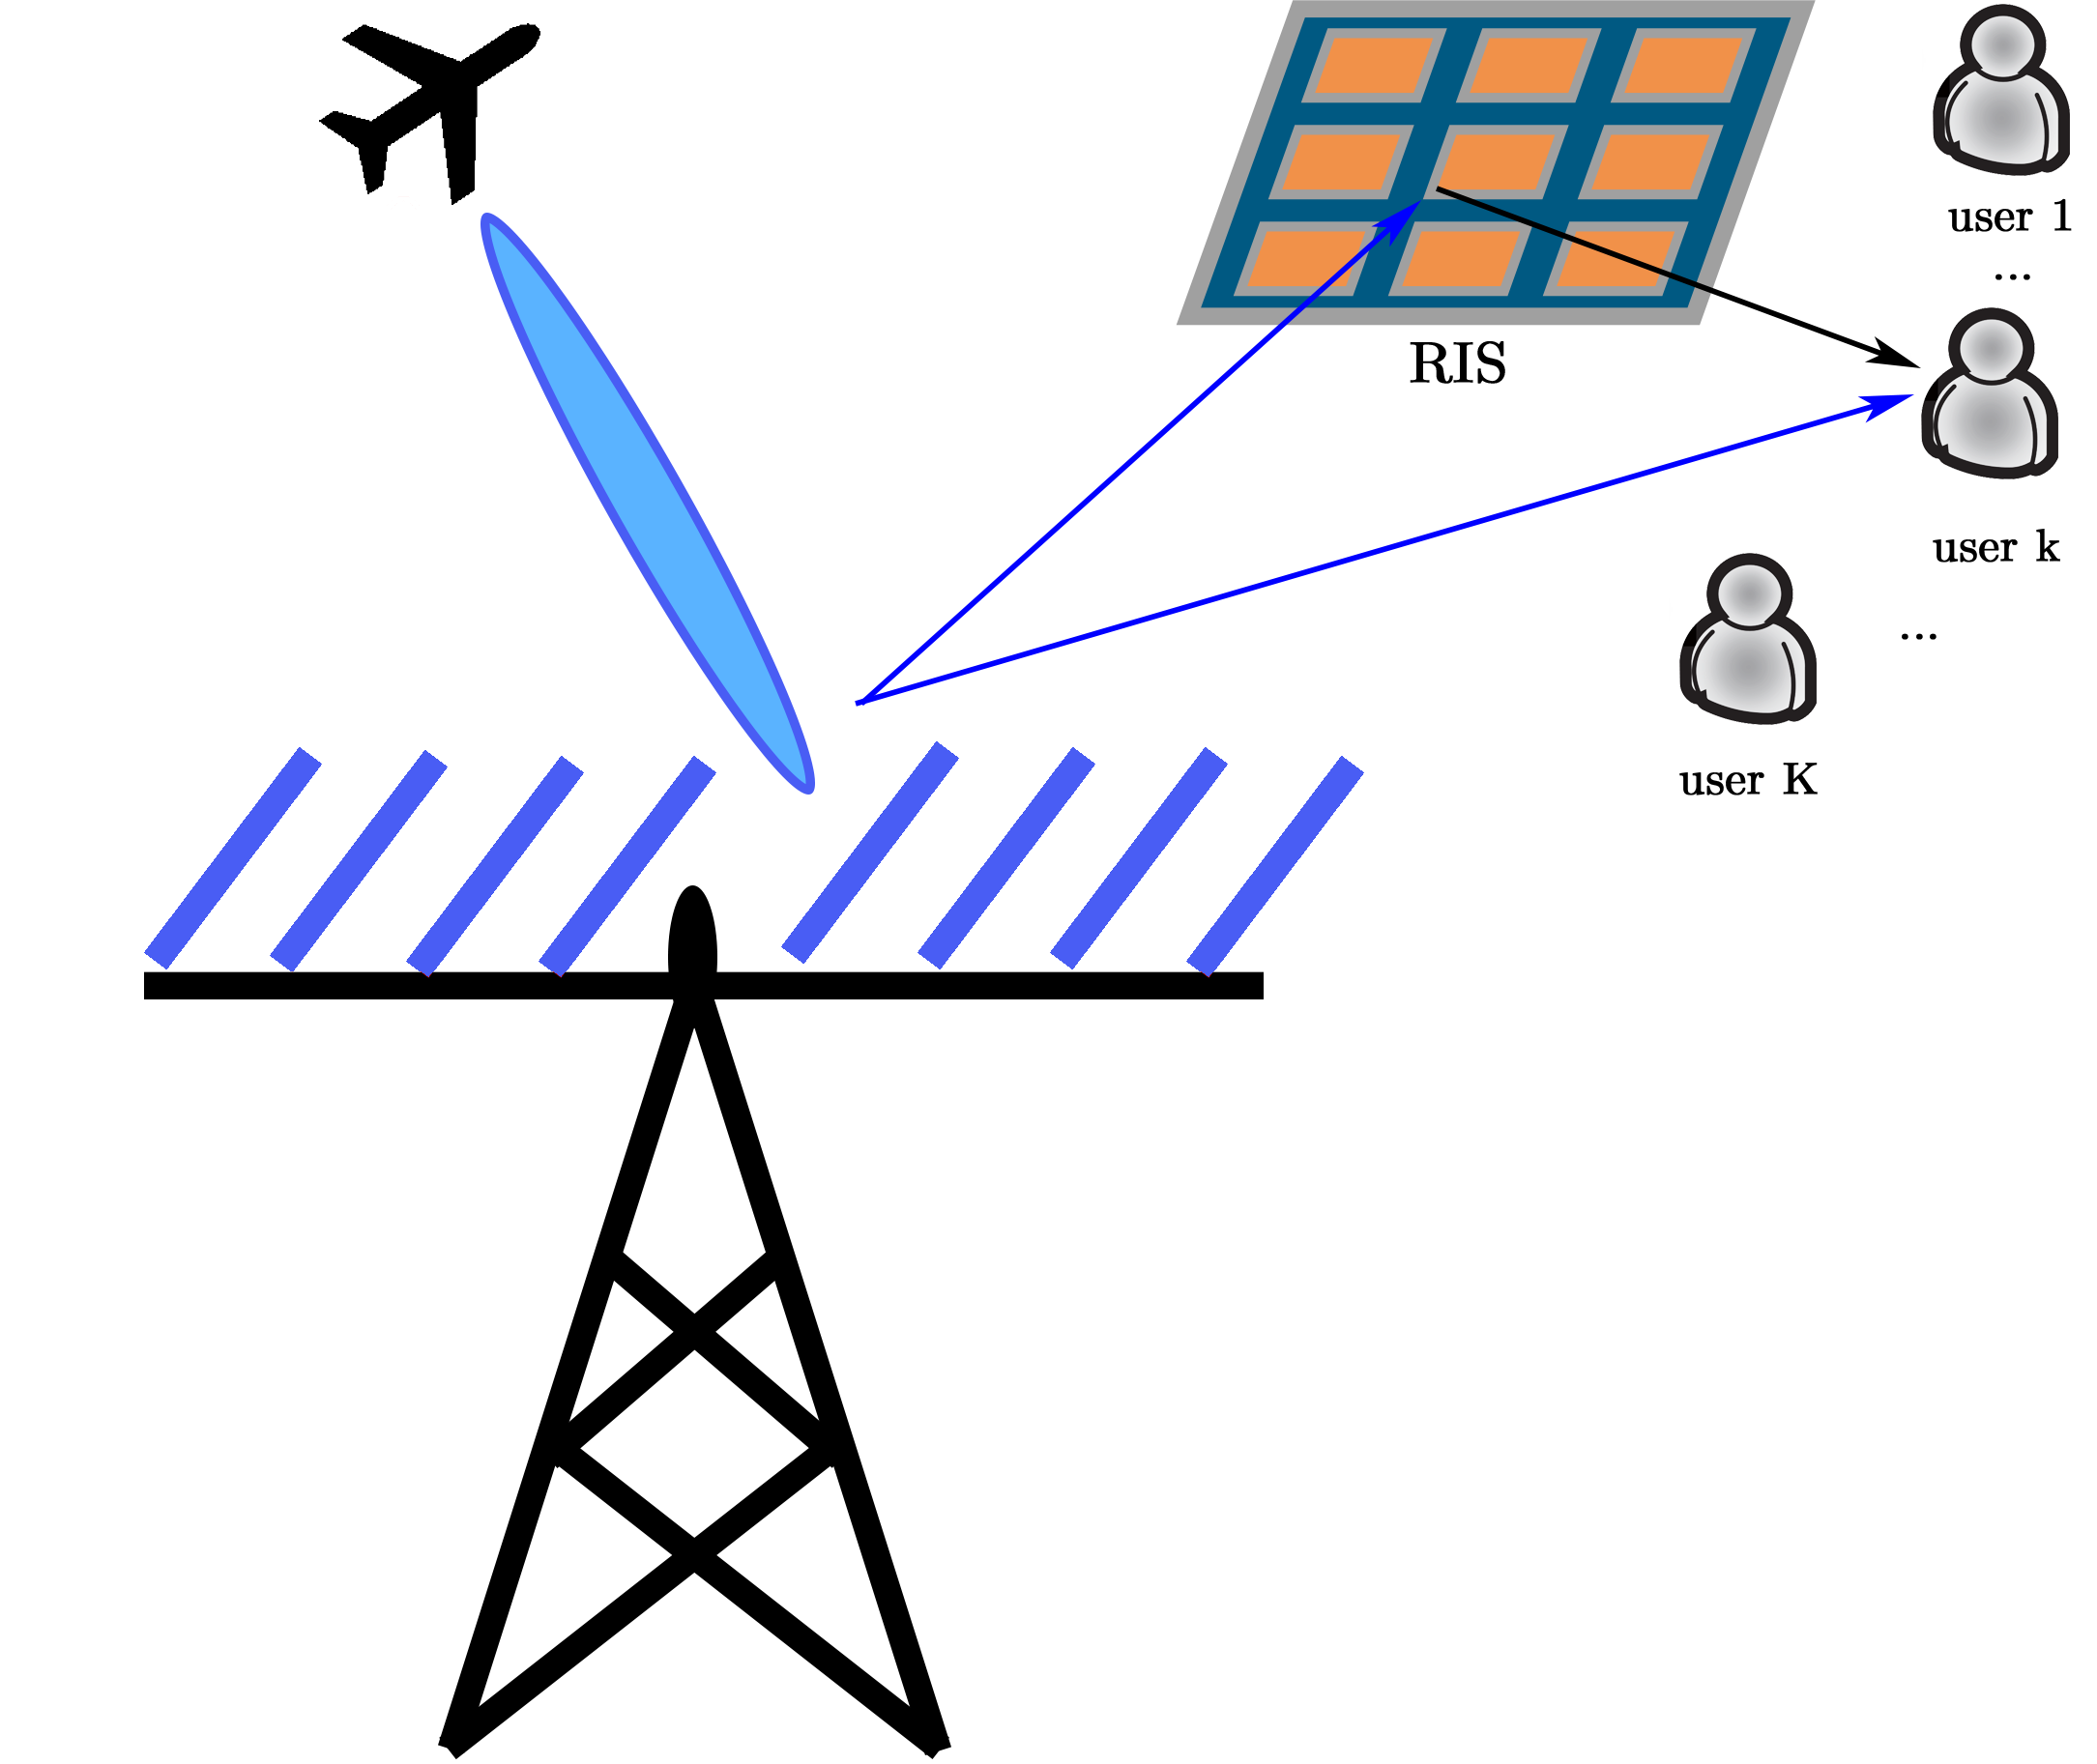
\includegraphics[width=0.42\textwidth]{./shared_setup.png}
        \label{fig:setup_shared}
    }
    \caption{RIS-aided Dual-functional Radar and Communication system}
    \label{fig:setup}
\end{figure}

Meanwhile, there is a high requirement of spectral efficiency (SE) and high energy efficiency (EE)
in next-generation (NG) communication networks due to the rapid expansion of modern techniques such as
multimedia and the Internet of Things (IoT).
In the past decade, Reconfigurable Intelligent Surface (RIS) is proposed as a 
potential technique to satisfy the SE and EE requirement.
RIS consists of many small reflecting elements, which can change the amplitude and/or phase of the electromagnetic waves 
to achieve the desired propagation characteristics \cite{liu2020RIS}. These reflecting elements are normally low-cost.
The reflecting coefficients (passive beamforming) at RIS can be controlled by the base 
station (BS) through the controllers. Therefore, in order to maximize the gain from RIS,
the beamforming at BS and  RIS are usually designed jointly. \cite{guo2019WSR,wu2019IRS,guo2020ris}.


In the DFRC system, there is usually a tradeoff between the radar and communications \cite{xu2020tradeoff}, which
means the performance of radar needs to be decreased to increase the performance of communications,
and vice versa. The RIS is capable of modifying the communication channel via passive beamforming,
which can provide extra capability for the communication functions in the DFRC system. Compared
with the DFRC without RIS, the RIS-aided DFRC has more capability (passive beamforming)
to achieve better communication performance when the radar performance is the same. Meanwhile, because of the 
tradeoff relationship, when the communication performance is the same, better radar performance can also be achieved in RIS-aided DFRC.
Therefore, by optimizing the active beamforming and passive beamforming, the overall performance of DFRC
can be enhanced.